\chapter{Background and Related Work}
\label{chap:background}

\section{Foundations of Productive Failure}
\label{sec:bg-pf-theory}

\subsection{Empirical Evidence for Productive Failure}
\label{subsec:bg-pf-evidence}
Kapur first introduced Productive Failure in a study on Newtonian kinematics~\cite{kapur2008}, where Grade~11 students worked in small groups on either ill-structured physics problems, which have missing information and several possible solutions, or well-structured problems. The groups working on ill-structured problems produced poorer solutions at first, but afterward they solved new problems of both types better than the other groups. Later studies moved from comparing two kinds of problems to comparing two whole teaching procedures, namely PF and direct instruction, where the formula is taught first. Kapur and Bielaczyc made this comparison for average speed~\cite{kapur2012}, and Kapur repeated it for variance~\cite{kapur2014}. These studies showed that the time spent struggling did not come at a cost: PF students calculated with the formula as well as students who had been taught it first, and they were even better at explaining why the formula works. A meta-analysis by Sinha and Kapur~\cite{sinha2021} confirmed this advantage across many studies and found it to be larger when the problem-solving phase closely follows PF design principles. 

\subsection{Learning Mechanisms and Design Principles}
\label{subsec:bg-pf-mechanisms}
Kapur and Bielaczyc~\cite{kapur2012} explain why PF works through four interdependent mechanisms, which describe the learning processes that PF aims to trigger in students. They derive the PF design principles from these mechanisms. Besides the requirements for the problem and the comparison of solutions in the second phase, which we described in Section~\ref{sec:intro-motivation}, these principles ask that students get room to explain and elaborate on their ideas. Each mechanism is supported by one or more of the principles.
\begin{enumerate}[label=(\alph*),leftmargin=0.9cm,itemsep=0.25em,topsep=0.3em]
    \item \emph{Activating prior knowledge:} Students apply what they already know to the problem and produce several different representations and solution methods. The problem itself supports this by building on that knowledge and allowing many approaches.
    \item \emph{Attending to the critical features of the concept:} Students' attention is drawn to the features that the target concept must capture, such as the spread of data around the mean for variance. All three principles support this mechanism.
    \item \emph{Explaining and elaborating on these features:} Students explain and elaborate on these features, first in their small groups while working on the problem and later in the whole-class discussion of their solutions.
    \item \emph{Assembling these features into the target concept:} Students organize these features into the target concept, which mainly happens when the teacher compares their solutions with the canonical one.
\end{enumerate}

For these four mechanisms to work, the problem must elicit several distinct attempts that each fail for a clear reason. Classroom studies show that students learn more when they generate more solutions in the first phase~\cite{kapur2023inventive} and when the teacher can point to the exact flaw in each attempt during the second phase~\cite{loibl2014}. Because group work and the classroom discussion remain the teacher's responsibility~\cite{kapur2012}, this thesis focuses on generating and evaluating the written problem itself.

\section{Generating Educational Tasks with LLMs}
\label{sec:bg-llm-math}

\subsection{Multiple-Choice Questions and Distractors}
\label{subsec:bg-llm-mcq}
An earlier use case of LLMs in educational task generation is creating multiple-choice questions (MCQs), where each wrong option, or distractor, is designed to match the answer a student reaches through a specific misconception rather than a random guess~\cite{alhazmi2024}. Large classroom datasets such as Eedi~\cite{wang2021eedi} support this by providing thousands of math questions in which every distractor is paired with a teacher-written explanation of the underlying misconception.

Building on Eedi, Feng et al.~\cite{feng2024} tested how well LLMs can generate three distractors per question and measured the share of generated distractors that matched the three human-written Eedi options. When prompted with random example questions, the model matched only $23.6\%$ of the human distractors, and selecting from hand-written error rules or asking GPT-4 to reason step by step about likely student errors (CoT) brought only modest improvements ($27\text{--}30\%$). The highest match rate, $38.5\%$, was achieved by retrieving the three most similar training questions together with their teacher-written distractors and error explanations as few-shot examples (RAG). Even on routine questions, an LLM therefore cannot reliably guess student mistakes from direct prompting alone, and instead needs real examples of student errors.

\subsection{Applying LLMs to Productive Failure}
\label{subsec:bg-llm-pf}
More recently, researchers have started to bring LLMs to Productive Failure itself. Puech et al.~\cite{puech2025} introduced \textsc{StratL} to steer an LLM tutor during the first phase of PF so that it selects pedagogical intents, such as asking students to test or compare their ideas, instead of revealing the canonical solution. In a high-school field study on expert-designed PF tasks, steering the tutor more than doubled the average number of student-generated representations and solution methods on the consistency task ($1.0$ to $2.6$) and substantially raised students' independent reasoning scores compared with an unsteered LLM tutor. However, their system still requires a human-designed PF problem and its solution space to be given in advance.

To generate the PF problems themselves, Rahimi et al.~\cite{rahimi2025productivemath} developed \emph{ProductiveMath}, an application that prompts GPT-4o to create algebra PF problems from a single six-part prompt containing PF principles, the evaluation rubric, and five human-written PF examples (Figure~\ref{fig:rahimi-setup-rubric}a), and rates each generated problem from 1 to 3 across the five rubric dimensions shown in Figure~\ref{fig:rahimi-setup-rubric}b for a total score between 5 and 15. Across three studies, they found high agreement between human raters and GPT-4o acting as an automated rubric judge, although seven math teachers who reviewed the problems noted in interviews that the tasks still needed better difficulty calibration, simpler wording, and stronger PF support.

\begin{figure}[t]
    \centering
    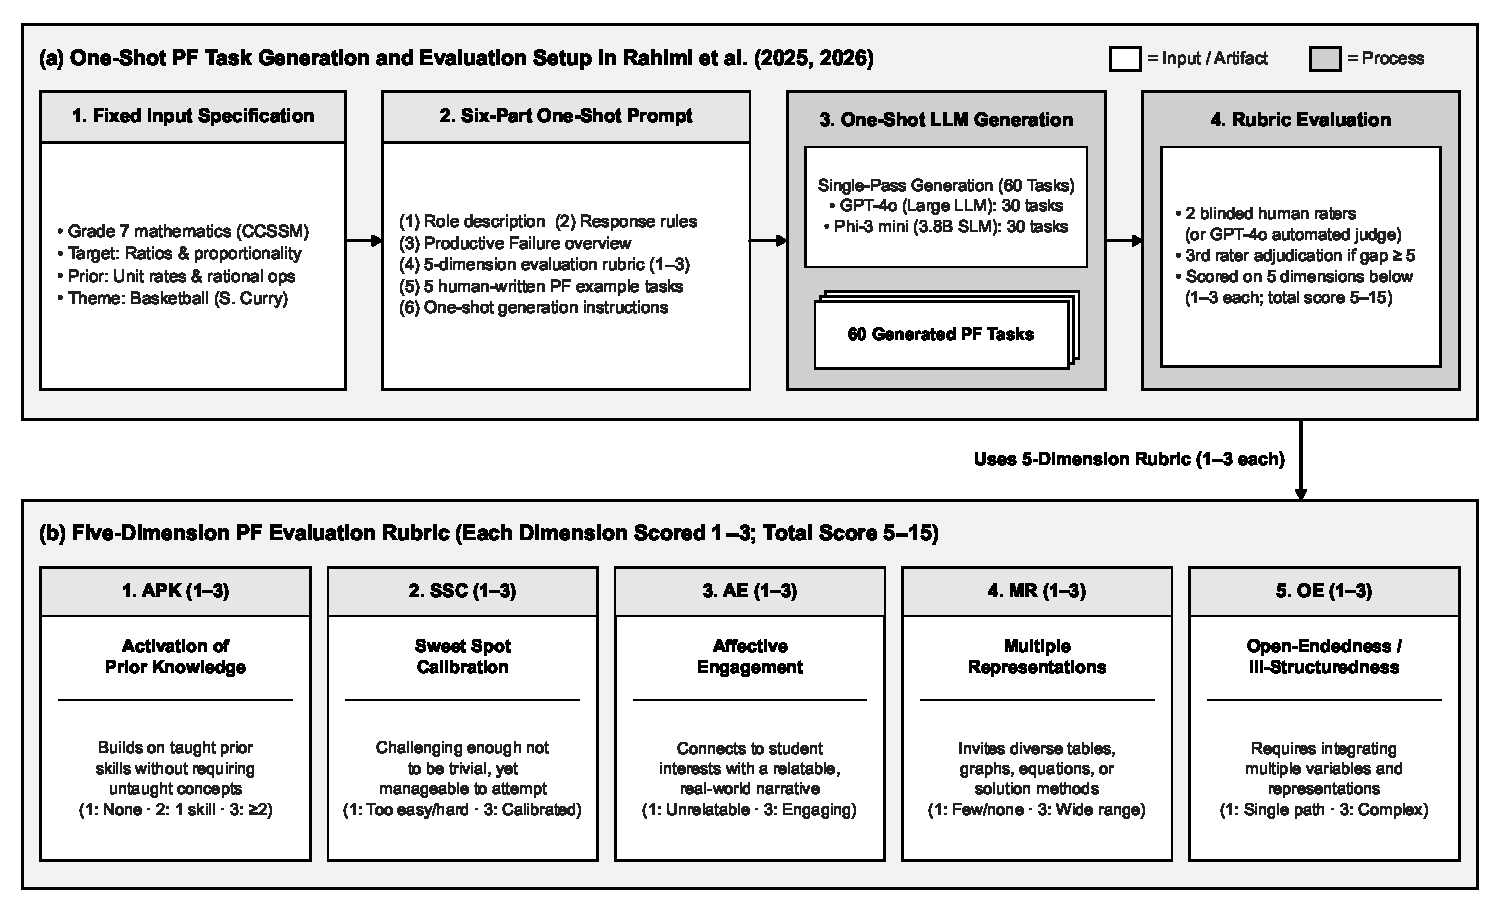
\includegraphics[width=\textwidth]{fig2_1_rahimi_setup_rubric.pdf}
    \caption[One-Shot Prompt (a) and Five-Dimension Rubric (b) from Rahimi et al.]{One-Shot Prompt~(a) and Five-Dimension Rubric~(b) from Rahimi et al.~\cite{rahimi2025productivemath,rahimi2025}}
    \label{fig:rahimi-setup-rubric}
\end{figure}

Because \emph{ProductiveMath} relied on a single large model (GPT-4o), Rahimi et al.~\cite{rahimi2025} next tested whether a small language model could match it under the same six-part prompt and rubric. They compared GPT-4o and Phi-3 mini (3.8B) on 60 problems (30 per model) generated for a single fixed setting targeting Grade~7 ratios and proportional relationships, with unit rates and rational-number operations as prior knowledge and a Stephen Curry basketball theme. As summarized in Table~\ref{tab:bg-rahimi-results}, two blinded human raters found that GPT-4o scored significantly higher than Phi-3 mini overall ($13.38$ vs.\ $10.67$ out of $15$, $d = 1.16$). While both models already scored high on affective engagement and prior-knowledge activation, GPT-4o more reliably followed the prompt's instructions to ask for diverse representations (such as tables, diagrams, and equations) and multi-path problem structures, driving large gains on multiple representations ($d = 1.65$) and open-endedness ($d = 1.58$).

\begin{table}[t]
\centering
\caption[Human Rubric Scores for GPT-4o and Phi-3 mini (Rahimi et al.)]{Human Rubric Scores for GPT-4o and Phi-3 mini (Rahimi et al.~\cite{rahimi2025})}
\label{tab:bg-rahimi-results}
\small
\setlength{\tabcolsep}{6pt}
\renewcommand{\arraystretch}{1.2}
\begin{tabular}{@{} l c c c @{}}
\toprule
\textbf{Rubric Dimension} & \textbf{GPT-4o ($n = 30$)} & \textbf{Phi-3 mini ($n = 30$)} & \textbf{Cohen's $d$} \\
\multicolumn{4}{@{}l}{\footnotesize\emph{Grade 7 ratios and proportional relationships, basketball theme; mean $\pm$ SD across two human raters}} \\
\midrule
Activation of Prior Knowledge (APK, 1--3) & $2.65 \pm 0.35$ & $2.42 \pm 0.53$ & $0.52$ \\
Sweet Spot Calibration (SSC, 1--3) & $2.52 \pm 0.55$ & $2.08 \pm 0.62$ & $0.74$ \\
Affective Engagement (AE, 1--3) & $2.75 \pm 0.47$ & $2.45 \pm 0.71$ & $0.50$ \\
Multiple Representations (MR, 1--3) & $2.70 \pm 0.43$ & $1.83 \pm 0.61$ & $1.65$ \\
Open-Endedness (OE, 1--3) & $2.77 \pm 0.47$ & $1.88 \pm 0.64$ & $1.58$ \\
\midrule
\textbf{Total Score (5--15)} & \textbf{13.38} $\pm$ \textbf{1.88} & \textbf{10.67} $\pm$ \textbf{2.73} & \textbf{1.16} \\
\bottomrule
\end{tabular}
\end{table}

\section{Evaluating Educational Tasks with LLMs}
\label{sec:bg-evaluation}

\subsection{Direct Rubric Scoring}
\label{subsec:bg-eval-rubrics}
Once educational tasks are generated automatically, evaluating every output with human teachers becomes a bottleneck. A common alternative is to use an LLM as an automated judge that reads the generated text and scores it on a Likert scale for each rubric dimension, a general evaluation approach popularized by \emph{G-Eval}~\cite{liu2023geval} and used for PF problems in \emph{ProductiveMath}~\cite{rahimi2025productivemath}. However, Liu et al.~\cite{liu2023geval}, Zheng et al.~\cite{zheng2023judging}, and Wang et al.~\cite{wang2024fairevaluators} show that such rubric-based LLM judges favor LLM-generated text and suffer from strong verbosity, formatting, and position biases, rewarding longer and more polished text even when the underlying content is flawed.

\subsection{Decomposed Checklists}
\label{subsec:bg-eval-checklists}
To make automated text evaluation more reliable, recent work replaces broad Likert scales with decomposed checklists. In \emph{CheckEval}, Lee et al.~\cite{lee2025checkeval} break each evaluation dimension into specific yes-or-no questions that the judge answers individually before scores are aggregated, which improves correlation with human raters and reduces scoring variance compared with direct Likert scales. Cook et al.~\cite{cook2024tick} report a similar advantage, showing that checklist items help judges catch specific omissions that direct rubric scores overlook. In education, Moore et al.~\cite{moore2023mcqquality} used GPT-4 to evaluate multiple-choice questions against a 19-item writing checklist, matching human raters on over $80\%$ of the criteria. However, their checklist only evaluates surface writing rules, such as clear phrasing and consistent option lengths, rather than the underlying mathematical structure or pedagogical design of the problem.

\subsection{Knowledge-Profile Student Simulation}
\label{subsec:bg-eval-simstudents-profile}
Instead of only inspecting the wording of a task, a second line of work evaluates educational items by having LLM-simulated students attempt them. In \emph{Generative Students}, Lu and Wang~\cite{lu2024} construct student profiles by specifying which knowledge components a learner has mastered, confuses, or does not know, and prompt simulated students to answer multiple-choice questions on user-interface design, matching college students' item-level performance well ($r = 0.72$). In a similar vein, Scarlatos et al.~\cite{scarlatos2025smart} in \emph{SMART} align simulated student responses with Item Response Theory to estimate the difficulty of reading and programming questions on held-out test items.

\subsection{Prior-Knowledge Leakage in Mathematics}
\label{subsec:bg-eval-simstudents}
When this persona-based approach is applied to mathematics, however, capable language models struggle to stay within a student's actual prior knowledge. Liu et al.~\cite{liu2023novice} tested GPT-4 on Eedi math questions and found that while the model solved $94.8\%$ of the problems correctly as an expert tutor, it could reproduce a specified student misconception on only $61.7\%$ of the items, often defaulting back to the correct calculation. Srivatsa et al.~\cite{srivatsa2025abilities} similarly found on national mathematics assessments (NAEP) that no model or persona prompt reliably matched real students' grade-level ability boundaries. Furthermore, Do, Sonkar, and Sachan~\cite{do2026faithfulness} showed that LLM student simulators abandon their initial errors under almost any follow-up prompt, even when the feedback is generic or unrelated to their mistake. Role-play student personas therefore cannot be trusted on their own to respect strict prior-knowledge limits on open math problems.

\section{Summary and Research Gap}
\label{sec:bg-gap}

\begin{table}[!htb]
\centering
\caption[Prior LLM Studies on Educational Task Generation and Evaluation]{Prior LLM Studies on Educational Task Generation and Evaluation}
\label{tab:bg-llm-comparison}
\footnotesize
\setlength{\tabcolsep}{3.5pt}
\renewcommand{\arraystretch}{1.35}
\begin{tabular}{@{} l l c c c @{}}
\toprule
\textbf{Study} & \textbf{Focus} & \textbf{Open PF Tasks} & \textbf{Prior Knowledge} & \textbf{Method-Failure Check} \\
\midrule
Feng et al.~\cite{feng2024} & MCQ distractors & -- & $\checkmark$ (error RAG) & -- \\
\addlinespace[3pt]
Lu and Wang~\cite{lu2024}; Liu et al.~\cite{liu2023novice} & Student simulation & -- & $\checkmark$ (persona profile) & -- \\
\addlinespace[3pt]
Puech et al.~\cite{puech2025} (\textsc{StratL}) & PF Phase~1 tutoring & -- & $\checkmark$ (expert-supplied) & -- \\
\addlinespace[3pt]
Rahimi et al.~\cite{rahimi2025productivemath,rahimi2025} & PF task generation & $\checkmark$ (one-shot) & -- & -- (surface rubric) \\
\midrule
\textbf{This thesis (\textsc{StructPF})} & \textbf{PF task generation} & \textbf{$\checkmark$ (3-stage)} & \textbf{$\checkmark$ (curriculum graph)} & \textbf{$\checkmark$ (calculator + solver)} \\
\bottomrule
\end{tabular}
\end{table}

Table~\ref{tab:bg-llm-comparison} summarizes how prior work relates to this thesis. On the generation side, MCQ distractor studies such as Feng et al.~\cite{feng2024} show that LLMs cannot reliably guess student mistakes from direct prompting alone and perform much better when given external information about student errors. However, MCQ generation only targets single-step mistakes on routine questions and does not capture the complexity of PF, where an open problem must let students try and compare several prior methods. Existing work on PF task generation targets open problems directly, but has only studied one-shot prompting on a narrow set of Grade~7 algebra topics, relying on the model's general ability to invent the scenario, numbers, and wording in a single pass~\cite{rahimi2025productivemath,rahimi2025}. On the evaluation side, prior PF studies score generated tasks on a surface level with a broad 1--3 rubric without testing whether familiar methods actually fail on the problem's numbers, while unconstrained role-play student simulators often solve problems using knowledge beyond the student's grade~\cite{liu2023novice,srivatsa2025abilities}. Given these limitations of one-shot prompting, surface rubrics, and unconstrained student simulation, this thesis investigates whether decomposing task design into curriculum-grounded, calculator-checked stages and evaluating the PF requirements directly can produce working PF tasks across a much broader range of mathematics topics and grade levels.
